\section{供电与用电}

\subsection{三相电源}

三相电源:三个正弦的感应电动势,互相间隔$120^\circ$,幅值相等,频率相同。\\
瞬时表达式:
\begin{equation}
    \begin{aligned}
        u_{1} &= U_m \sin \omega t \\
        u_{2} &= U_m \sin (\omega t - 120^\circ) \\
        u_{3} &= U_m \sin (\omega t + 120^\circ)
    \end{aligned}
\end{equation}
\noindent 相量表达式:
\begin{equation}
    \begin{aligned}
        \dot{U}_{1} &= U_m \phase{ 0^\circ }\\
        \dot{U}_{2} &= U_m \phase{ -120^\circ} \\
        \dot{U}_{3} &= U_m \phase{ 120^\circ}
    \end{aligned}
\end{equation}

%波形图和相量图
\begin{figure}[!ht]
    \centering
    \begin{minipage}[t]{0.4\linewidth}
        \centering
        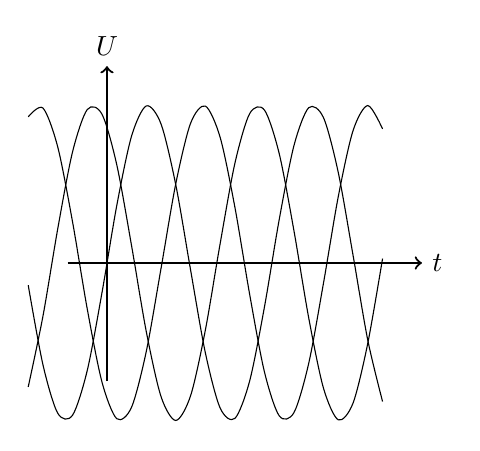
\begin{tikzpicture}
            %\draw[very thin,color=gray] (-0.1,-1.1) grid (3.9,8.1);
            \draw[->,thick] (-0.5,0) -- (4,0) node[right] {$t$};
            \draw[->,thick] (0,-1.5) -- (0,2.5) node[above] {$U$};
            
            \draw[domain=-1:3.5,smooth] plot(\x,{2*sin(3*\x r + 120)});
            \draw[domain=-1:3.5,smooth] plot(\x,{2*sin(3*\x r - 120)});
            \draw[domain=-1:3.5,smooth] plot(\x,{2*sin(3*\x r )});
        
        \end{tikzpicture}
    \caption{波形图}
    \end{minipage}
    \begin{minipage}[t]{0.4\linewidth}
        \centering
        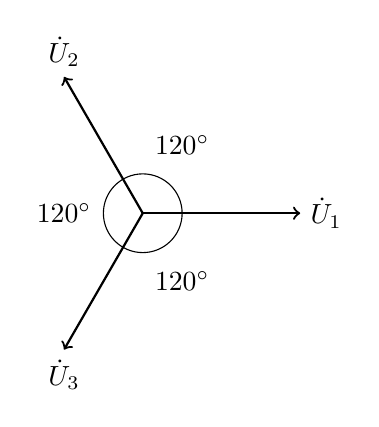
\begin{tikzpicture}
            %\draw[very thin,color=gray] (-0.1,-1.1) grid (3.9,8.1);
            \draw[->,thick] (0,0) -- (2,0) node[right] {$\dot{U}_{1}$};
            \draw[->,thick] (0,0) -- (-1,1.732) node[above] {$\dot{U}_{2}$};
            \draw[->,thick] (0,0) -- (-1,-1.732) node[below] {$\dot{U}_{3}$};
            %\draw (0.5,0) arc (0:120:0.5) node[right] {$120^\circ$};
            %\draw (0.5,0) arc (0:-120:0.5) node[right] {$120^\circ$};
            \draw (0,0) circle (0.5);
            \node at (0.5,0.866) {$120^\circ$};
            \node at (0.5,-0.866) {$120^\circ$};
            \node at (-1,0) {$120^\circ$};
        \end{tikzpicture}
        \caption{向量图}
    \end{minipage}
\end{figure}

\subsubsection{三相电源的星形联结}

如下图所示,三相绕组的三个末端接在一起,与三个首段一起向外引出
四根供电线,或只从三个首段引出三根供电线,称为三相电源的星形联结。
前者称作三相四线制,后者称作三相三线制。

\begin{center}
    \begin{circuitikz}[american voltages]
        \draw
        (0,0) node[anchor=east] {N}
        to [american inductor, *-] (0,2)
        to [short, -o] (5,2) node[anchor=west] {$\text{L}_1$} ;
        \draw
        (0,0)
        to [short, -o] (5,0) node[anchor=west] {$\text{N}$} ;
        \draw
        (0,0)
        to [american inductor, *-] (1.732,-1)
        to [short, -o] (5,-1) node[anchor=west] {$\text{L}_2$} ;
        \draw
        (0,0)
        to [american inductor, *-] (-1.732,-1)
        to [short] (-1.732,-2) 
        to [short, -o] (5,-2) node[anchor=west] {$\text{L}_3$} ;
    \end{circuitikz}
\end{center}

N为中性点,引出的导线称为中性线,又称零线。
由L1、L2、L3引出的导线称为相线或端线,俗称火线。\\
相电压:相线与中位线之间的电压,用$U_{1},U_2,U_3$表示。\\
线电压:两相线之间的电压,用$U_{12},U_{23},U_{31}$表示。

\begin{equation}
    \begin{aligned}
        \dot{U}_{12} &= \dot{U}_{1} - \dot{U}_{2} \\
        \dot{U}_{23} &= \dot{U}_{2} - \dot{U}_{3} \\
        \dot{U}_{31} &= \dot{U}_{3} - \dot{U}_{1}
    \end{aligned}
\end{equation}

\noindent 用$U_P$表示相电压有效值,$U_L$表示线电压有效值,电压对称情况下有:

\begin{equation}
        U_l=\sqrt{3}U_P
\end{equation}

\noindent 相电流:每相绕组的电流,用$I_1,I_2,I_3$表示。

\noindent 线电流:端点输出的电流,用$I_{L1},I_{L2},I_{L3}$表示。

\begin{equation}
    \begin{aligned}
        \dot{I}_{L1} &= \dot{I}_{1} \\
        \dot{I}_{L2} &= \dot{I}_{2} \\
        \dot{I}_{L3} &= \dot{I}_{3}
    \end{aligned}
\end{equation}

\noindent 用$I_P$表示相电流有效值,$I_L$表示线电流有效值,电流对称情况下有:

\begin{equation}
        I_l=I_P
\end{equation}

\subsubsection{三相电源的三角联结}

如下图所示,三相电源中的每相绕组首尾相接,形成一个闭合回路,
然后从连接点引出三根供电线,这种连接方式称为三相电源的三角联结。

\begin{center}
    \begin{circuitikz}[american voltages]
        \draw
        (-1.732,-1)
        to [american inductor, i=$\dot{I}_{1}$, *-] (0,2)
        to [short, -o] (5,2) node[anchor=west] {$\text{L}_1$} ;
        \draw
        (0,2)
        to [american inductor, i=$\dot{I}_{2}$, *-] (1.732,-1)
        to [short, -o] (5,-1) node[anchor=west] {$\text{L}_2$} ;
        \draw
        (1.732,-1)
        to [american inductor, i=$\dot{I}_{3}$, *-] (-1.732,-1)
        to [short] (-1.732,-2) 
        to [short, -o] (5,-2) node[anchor=west] {$\text{L}_3$} ;
    \end{circuitikz}
\end{center}

\noindent 相电压与线电压的关系以及相电流与线电流的关系

\begin{equation}
    \begin{aligned}
        \dot{U}_{1} &= \dot{U}_{12} \\
        \dot{U}_{2} &= \dot{U}_{23} \\
        \dot{U}_{3} &= \dot{U}_{31}
    \end{aligned}
\end{equation}
\begin{equation}
    \begin{aligned}
        \dot{I}_{L1} &= \dot{I}_{1} - \dot{I}_{2} \\
        \dot{I}_{L2} &= \dot{I}_{2} - \dot{I}_{3} \\
        \dot{I}_{L3} &= \dot{I}_{3} - \dot{I}_{1}
    \end{aligned}
\end{equation}



\subsection{三相负载}

\noindent 每相负载首末端之间的电压称为相电压。\\
两相负载首端之间的电压称为线电压。

\noindent 相电压与相电流之间的关系

\begin{equation}
    \begin{aligned}
        \dot{U}_{1} &= \dot{Z}_{1} \dot{I}_{1} \\
        \dot{U}_{2} &= \dot{Z}_{2} \dot{I}_{2} \\
        \dot{U}_{3} &= \dot{Z}_{3} \dot{I}_{3}
    \end{aligned}
\end{equation}

\noindent \textbf{对称三相电路中,中性线的电流为零。\\
中性线的作用:保持负载中性点和电源中性点电位相同。从而在
三相负载不对称时,负载的相电压仍是对称的。}


\subsection{触电防护}

了解安全电压,保护接地、保护接零(IT系统,TN系统,TT系统),漏电开关。
